
% This LaTeX was auto-generated from MATLAB code.
% To make changes, update the MATLAB code and republish this document.

\documentclass{article}
\usepackage{graphicx}
\usepackage{color}

\sloppy
\definecolor{lightgray}{gray}{0.5}
\setlength{\parindent}{0pt}

\begin{document}

    
    

\section*{25. Two famous problems}

\begin{verbatim}
ATAPformats
\end{verbatim}
\begin{par}
In this chapter we discuss two problems of rational approximation that have been the focus of special attention over the years: approximation of $|x|$ on $[-1,1]$, a prototype of approximation of non-smooth functions, and approximation of $e^x$ on $(-\infty,0\kern .5pt ]$, a prototype of approximation on unbounded domains.  Both stories go back many decades and feature initial theorems, later conjectures based on numerical experiments, and eventual proofs of the conjectures based on mathematical methods related to potential theory. We shall not present the proofs of the sharpest results, but we shall show that the essential rates of approximation can be achieved by using the trick that appears several times in this book: if a function $f(x)$ can be written as an integral with respect to a variable $s$, then an approximation $r(x)$ in partial fractions form is obtained by applying a quadrature formula (19.3) to the integral.
\end{par} \vspace{1em}
\begin{par}

The problem of approximation of $|x|$ on $[-1,1]$ originates at the beginning
of the 20th century, when polynomial approximations of this function were
of interest to Lebesgue, de la $\hbox{Vall\'ee}$ Poussin, Jackson, and
Bernstein.  This was an era when the fundamental results of
approximability were being developed, and $|x|$ served as a function from
which many other results could be derived.  Bernstein's prize-winning
article on the subject ran for 104 pages [1912{\sc b}] and was followed
by another of 57 pages [1914{\sc b}].  Among other
things, Bernstein proved that in best polynomial approximation of $|x|$
as $n\to\infty$, the errors decrease linearly but no faster, that
is, at the rate $O(n^{-1})$ but not $o(n^{-1})$.

\end{par} \vspace{1em}
\begin{par}
Why linearly?  This is an example of the fundamental fact of approximation theory which we mentioned first in Chapter 7: the close connection between the smoothness of a function and its rate of approximation.  The function $f(x) = |x|$ has a derivative of bounded variation $V=2$ on $[-1,1]$, so by Theorem 7.2, its Chebyshev projections $\{f_n\}$ satisfy $$ \| f-f_n \| \le {4\over \pi (n-1)} $$ for $n\ge 2$, and its Chebyshev interpolants $\{p_n\}$ satisfy the same bound with 4 replaced by 8.  Thus approximations to $|x|$ converge at least at the rate $O(n^{-1})$.  What Bernstein showed is that the rate is in fact no better than this: no approximations to $|x|$ can beat Chebyshev projection or interpolation by more than a constant factor.  Or to put it another way, convergence of polynomial approximants to a function $f$ at a rate faster than $O(n^{-1})$ implies that $f$ is in some sense smoother than $|x|$. Such results in the direction \textit{approximability} $\Longrightarrow$ \textit{smoothness} go by the general name of \textit{Bernstein theorems}.  In this book we have presented one result of this kind: Theorem 8.3, asserting that geometric convergence implies analyticity.
\end{par} \vspace{1em}
\begin{par}

It is hard not to be curious about the constants. Bernstein in fact
proved in [Bernstein 1914{\sc b}] that there exists a number $\beta$ such that
the best approximation errors satisfy
$$ E_n (|x|) \sim {\beta\over n} \eqno (25.1) $$
as $n\to\infty$, and he obtained the bound
$$ 0.278 < \beta < 0.286. $$
(Theorem 7.2 gives $\beta \le 4/\pi \approx 1.27$.) He noted as a ``curious
coincidence'' that
$1/2\sqrt \pi \approx 0.28209\dots$ falls in this range, and the idea
that $\beta$ might take exactly this value
became known as {\em Bernstein's conjecture.}  Seventy years later, Varga and
Carpenter [1985] investigated the problem numerically to great accuracy
and found that in fact
$$ \beta \approx 0.28016949902386913303643649\dots. $$
(Of course the difference between 0.282 and 0.280 would not have the
slightest practical importance.)  Along with this numerical result, which
was based on Richardson extrapolation, Varga and Carpenter established
the rigorous bounds
$$ 0.2801685 < \beta < 0.2801734. \eqno (25.2) $$

\end{par} \vspace{1em}
\begin{par}
 \vskip -2.5em 
\end{par} \vspace{1em}
\begin{par}
For example, here are the values of $nE_n(|x|)$ for $n = 1,2,4, \dots, 64$, showing quadratic convergence to the limit value.  A comparison with the much more accurate Table 2.1 of [Varga \& Carpenter 1985] indicates that the Chebfun results are accurate in all but the last digit or two.
\end{par} \vspace{1em}
\begin{par}
 \vskip -2em 
\end{par} \vspace{1em}
\begin{verbatim}
x = chebfun('x'); f = abs(x); limit = 0.280169499023869133;
disp('            n           n*err        n*err - limit')
for n = 2.^(0:6)
  [p,err] = remez(f,n);
  fprintf('%14d %16.8f %16.2e\n',n,n*err,n*err-limit)
end
\end{verbatim}

        \color{lightgray} \begin{verbatim}            n           n*err        n*err - limit
             1       0.50000000         2.20e-01
             2       0.25000000        -3.02e-02
             4       0.27048360        -9.69e-03
             8       0.27751782        -2.65e-03
            16       0.27948884        -6.81e-04
            32       0.27999815        -1.71e-04
            64       0.28012659        -4.29e-05
\end{verbatim} \color{black}
    \begin{par}
Now all this is for polynomial approximation.  What about rational functions?  As mentioned in Chapter 23, the dramatic discovery here came from Donald Newman, fifty years after Bernstein: best rational approximants to $|x|$ converge ``root-exponentially''.  Newman's bounds were these: $$ {1\over 2} \kern .5pt e^{-9\sqrt n\kern 1pt} \le E_{nn}(|x|) \le 3\kern .5pt e^{-\sqrt n}. \eqno (25.3) $$ We have already seen in the second plot of Chapter 23 what an improvement in convergent rate this is as compared with (25.1). For approximating non-smooth functions, rational functions can be far more powerful than polynomials.
\end{par} \vspace{1em}
\begin{par}
Again mathematicians could not resist trying to sharpen the constants. First, Vyacheslavov [1975] found that the exact exponent is midway between Newman's bounds of 1 and 9: it is $\pi$.  Then Varga, Ruttan and Carpenter [1993] performed computations with a version of the Remez algorithm to 200 decimal places, leading to numerical evidence for the conjecture $$ E_{nn} \sim 8 \kern .5pt e^{-\pi \sqrt n } $$ as $n\to\infty$.  Soon afterwards this result was proved by Stahl [1993]. Later Stahl generalized the result to approximation of $x^\alpha$ on $[0,1]$ for any $\alpha>0$ [Stahl 2003].
\end{par} \vspace{1em}
\begin{par}
The following theorem summarizes the results we have mentioned.
\end{par} \vspace{1em}
\begin{par}

{\bf Theorem 25.1.  Approximation of \boldmath $|x|$ on $[-1,1]$.} {\em
The errors in best polynomial and rational approximation of $|x|$ on
$[-1,1]$ satisfy as $n\to\infty$
$$ E_{n0}(|x|) \sim {\beta\over n}, \quad \beta = 0.2801\dots \eqno (25.4) $$
and
$$ E_{nn}(|x|) \sim 8\kern .5pt e^{-\pi\sqrt n}. \eqno (25.5) $$}
\vskip -1em

\end{par} \vspace{1em}
\begin{par}
\textit{Proof.} Equation (25.4) is due to Varga and Carpenter [1985] and (25.5) is due to Stahl [1993]. $~\hbox{\vrule width 2.5pt depth 2.5 pt height 3.5 pt}$
\end{par} \vspace{1em}
\begin{par}
\textit{Why} can rational approximations of $|x|$ achieve $O(C^{-\sqrt n}\kern 1pt)$ accuracy?  The crucial fact is that the poles of $r$ can be chosen to cluster near the singular point $x=0$.  In particular, a good choice is to make the poles approach $0$ geometrically, for each fixed $n$, with a geometric factor depending on $\sqrt n$.
\end{par} \vspace{1em}
\begin{par}
Here is a derivation of a rational approximation that achieves the right root-exponential convergence.  (Arguments like this have been made by Stenger in various publications; see for example [Stenger 1986].) We start from the identity $$ {1\over |x|} = {2\over \pi} \int_0^\infty {dt\over t^2 + x^2}, $$ which is derived in calculus courses.  Multiplying by $x^2$ gives $$ |x| = {2x^2\over \pi} \int_0^\infty {dt\over t^2+x^2}. \eqno (25.6) $$ (This formula is perhaps due to Roberts [1980], though the essence of the matter dates to Zolotarev in the 1870s.) The change of variables $t = e^s$, $dt = e^s ds$ converts this to $$ |x| = {2x^2\over \pi} \int_{-\infty}^\infty {e^s ds\over e^{2s}+x^2}, \eqno (25.7)  $$ which is an attractive integral to work with because the integrand decays exponentially as $|s|\to\infty$. We now get a rational approximation of $|x|$ by approximating this integral by the trapezoid rule with node spacing $h>0$: $$ r(x) = {2hx^2\over \pi} \sum_{k = -(n-2)/4}^{(n-2)/4} {e^{kh}\over e^{2kh} + x^2}. \eqno (25.8) $$ Here $n$ is a positive even number, and there are $n/2$ terms in the sum, so $r(x)$ is a rational function of $x$ of type $(n,n)$. There are two sources of error that make $r(x)$ differ from $|x|$. The fact that the sum has been terminated at a limit $n<\infty$ introduces an error on the order of $e^{-nh/4}$, and the finite step size $h>0$ introduces an error on the order of $e^{-\pi^2/h}$.  (The integrand is analytic in the strip around the real $s$-axis of half-width $a=\pi/2$, corresponding to a convergence rate $e^{-2\pi a/h}$.) Balancing these sources of error suggests the condition $e^{-nh/4} \approx e^{-\pi^2/h}$, that is, $$ h \approx 2\pi/\sqrt n, \eqno (25.9) $$ with error of order $$ e^{-(\pi/2) \sqrt n}. \eqno (25.10) $$
\end{par} \vspace{1em}
\begin{par}
We can see these approximations with an experiment.
\end{par} \vspace{1em}
\begin{par}
 \vskip -2em 
\end{par} \vspace{1em}
\begin{verbatim}
for n = 2:2:12
  r = 0*x; h = 2*pi/sqrt(n);
  for k = -(n-2)/4:(n-2)/4
    r = r + exp(k*h)./(exp(2*k*h)+x.^2);
  end
  r = (2*h/pi)*x.^2.*r; err = norm(f-r,inf);
  subplot(3,2,n/2), plot(r), ylim([0 1])
  ss = sprintf('(%1d,%1d)   error = %5.3f',n,n,err);
  FS = 'fontsize'; text(-.5,.78,ss,FS,8)
end
\end{verbatim}

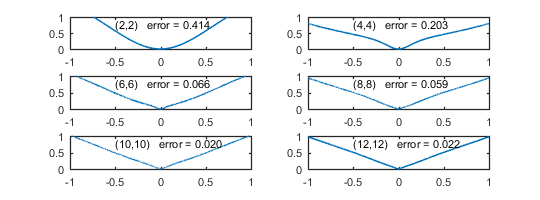
\includegraphics [width=4in]{chap25_01.png}
\begin{par}
 \vskip 1pt 
\end{par} \vspace{1em}
\begin{par}
The poles of (25.8)--(25.9) in the $x$-plane lie at $$ \pm i \kern .5pt e^{2\pi k/\sqrt n}. \eqno (25.11) $$ Here are these numbers (those in the upper half-plane) for the six approximations plotted above, showing the wide range of amplitudes associated with the exponential spacing.
\end{par} \vspace{1em}
\begin{par}
 \vskip -2em 
\end{par} \vspace{1em}
\begin{verbatim}
disp('Poles of rational approximants to |x|:')
for n = 2:2:12
  h = 2*pi/sqrt(n); k = -(n-2)/4:(n-2)/4; y = exp(k*h);
  fprintf('%8.2ei  ',y), disp(' ')
end
\end{verbatim}

        \color{lightgray} \begin{verbatim}Poles of rational approximants to |x|:
1.00e+00i   
2.08e-01i  4.81e+00i   
7.69e-02i  1.00e+00i  1.30e+01i   
3.57e-02i  3.29e-01i  3.04e+00i  2.80e+01i   
1.88e-02i  1.37e-01i  1.00e+00i  7.29e+00i  5.32e+01i   
1.07e-02i  6.58e-02i  4.04e-01i  2.48e+00i  1.52e+01i  9.32e+01i   
\end{verbatim} \color{black}
    \begin{par}
The approximations aren't optimal, but they are close.  The convergence rate (25.10) as $n\to\infty$ is one-quarter of the optimal rate (25.5) in the sense that we need $4$ times as large a value of $n$ to achieve a certain accuracy in (25.10) as in (25.5).
\end{par} \vspace{1em}
\begin{par}
Above, we computed errors for best polynomial approximations to $|x|$ with the Chebfun command \texttt{remez}.  In the rational case, \texttt{remez} does not succeed in computing best approximations beyond a certain low order. This difficulty is related to the exponential spacing of the oscillations of $f-r^*$ near $x=0$.
\end{par} \vspace{1em}
\begin{par}
It is worth noting that the problem of approximating $|x|$ on $[-1,1]$ is equivalent to certain other approximation problems. If $r(x)$ is a type $(m,n)$ approximation to $|x|$ on $[-1,1]$, then normally $r$ will be an even function of $x$ and $m$ and $n$ can be taken to be even too. Thus $r(x) = \tilde r (x^2)$, where $\tilde r$ is a rational function of type $(m/2,n/2)$.  Since $\tilde r(x^2)$ approximates $|x|$ for $x\in [-1,1]$, $\tilde r(x)$ approximates $\sqrt x$ for $x\in [0,1]$.  This reasoning holds for any approximations, and in particular, by counting equioscillations one finds that best type $(m,n)$ approximation of $|x|$ on $[-1,1]$ is equivalent to best type $(m/2,n/2)$ approximation of $\sqrt x$ on $[0,1]$. The following pair of plots illustrates this equivalence.  Notice that the error curves are the same apart from the scaling of the $x$-axis.
\end{par} \vspace{1em}
\begin{par}
 \vskip -2em 
\end{par} \vspace{1em}
\begin{verbatim}
f = abs(x); [p,q,rh,err] = remez(f,2,2); clf
subplot(1,2,1), plot(f-p./q), hold on, ylim(.08*[-1 1])
plot([-1 1],err*[1 1],'--k'), plot([-1 1],-err*[1 1],'--k')
title('Error in type (2,2) approx to |x|',FS,9)
f = chebfun('sqrt(x)',[0,1],'splitting','on');
[p,q,rh,err] = remez(f,1,1);
subplot(1,2,2), plot(f-p./q), hold on, axis([-.03 1 .08*[-1 1]])
plot([-.03 1],err*[1 1],'--k'), plot([0 1],-err*[1 1],'--k')
title('Error in type (1,1) approx to sqrt(x)',FS,9)
\end{verbatim}

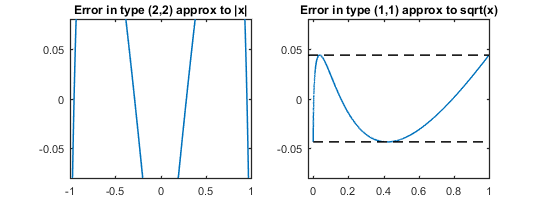
\includegraphics [width=4in]{chap25_02.png}
\begin{par}
 \vskip 1pt 
\end{par} \vspace{1em}
\begin{par}
For applications in scientific computing, the approximation of $\sqrt x$ on an interval $[a,b]$ is particularly interesting because of the case in which $x$ is a matrix $A$ with eigenvalues in $[a,b]$, which might come from discretizing a differential operator.  Rational approximations of the square root lead to powerful algorithms for evaluating $A^{1/2} v$ for vectors $v$, as described in [Hale, Higham \& Trefethen 2008] and [Higham 2008]. At the other end of the historical spectrum, approximation of square roots was the problem addressed by Poncelet in the very first paper on minimax approximation [Poncelet 1835].
\end{par} \vspace{1em}
\begin{par}
 We now turn to the second of the famous problems of this chapter:
approximation of $e^x$ on $(-\infty,0\kern .5pt ]$.  This problem was
introduced in a paper of Cody, Meinardus and Varga [1969], which drew
attention to the connection of such approximations with the numerical
solution of partial differential equations, since a rational
approximation can be used to compute the exponential of a matrix arising
from a numerical discretization [Moler \& Van Loan 2003].\footnote{The
Cody--Meinardus--Varga paper was important in my life.  As a graduate
student in the Numerical Analysis Group at Stanford, I happened to come
across it one evening around 1980 in a pile of Gene Golub's discarded
reprints---``help yourself''. Its mix of theory and numerical
calculations appealed to me greatly and led to my computation of the
constant $9.28903\dots$ a few years later [Trefethen \& Gutknecht
1983b].}  Curiously, despite that good motivation from applied
mathematics, the influence of this paper was mainly in theoretical
approximation theory for quite a few decades, until computers and
numerical linear algebra had advanced to the point where it became more
practical to take advantage of algorithms based on rational functions.

\end{par} \vspace{1em}
\begin{par}
The first thing we may note about approximation of $e^x$ on $(-\infty,0\kern .5pt ]$ is that polynomials cannot do the job at all. Since any non-constant polynomial $p(x)$ diverges to $\pm \infty$ as $x\to-\infty$, the only polynomials that can approximate $e^x$ with finite error on $(-\infty,0\kern .5pt ]$ are constants, so the minimax error can never be less than $1/2$.
\end{par} \vspace{1em}
\begin{par}

Inverse-polynomials of the form $1/p_n(x)$, however, can be chosen to
converge geometrically.  This makes sense when you consider that $e^{x}$
on $(-\infty,0\kern .5pt ]$ is the same as $1/e^x$ for $x\in[0,\infty)$.
Cody, Meinardus and Varga noted that to achieve geometric convergence, it
is enough to consider $1/p_n(x)$, where $p_n$ is the degree-$n$
truncation of the Taylor series for $e^x$. They showed that these
approximations converge at a rate $O(2^{-n})$, and then they improved
this rate to $O(2.298^{-n})$ by a shift of origin.  It was later proved
by Sch\"onhage [1973] that the optimal rate for inverse-polynomials is
$O(3^{-n})$.

\end{par} \vspace{1em}
\begin{par}

Since $1/p_n(x)$ is a rational function of type $(n,n)$, these
observations tell us that best rational type $(n,n)$ approximations to
$e^x$ on $(-\infty,0\kern .5pt ]$ converge at least geometrically. Newman
[1974] proved that the convergence is no faster than geometric. What is
the optimal rate?  With twice as many parameters to work with as with
inverse-polynomials, one might guess that it should be $O(9^{-n})$, and
this idea became known in the 1970s as the {\em $1/9$ conjecture.} In fact,
the optimal convergence rate turned out to be $O(H^{n})$ with $H \approx
1/9.28903,$ a number now known as {\em Halphen's constant}, equal to the
unique positive root of the equation
$$ h(s) = \sum_{k=1}^\infty {ks^n\over 1 - (-s)^n} = {1\over 8}.
\eqno(25.12) $$
This number was conjectured numerically based on Carath\'eodory--Fej\'er
singular values by Trefethen and Gutknecht [1983{\sc b}], verified to many
digits by high-precision Remes algorithms by Carpenter, Ruttan and Varga
[1984], conjectured to have the exact value associated with a certain
problem of elliptic functions treated by Halphen [1886] by Magnus via the
Carath\'eodory--Fej\'er method [Magnus 1985, Magnus \& Meinguet 2000],
and then proved using quite
different methods of potential theory by Gonchar and Rakhmanov [1989].
This work represents a fascinating and important line of investigation in
approximation theory, and for a summary of many of the ideas with
wide generalizations to related problems, a good place to start is [Stahl \&
Schmelzer 2009]. Presentations of some of the potential theory underlying
results in this area can be found in [Saff \& Totik 1997].

\end{par} \vspace{1em}
\begin{par}

Following the idea presented earlier for $|x|$ on $[-1,1]$, it is
interesting to see what can be achieved for this problem by the trapezoid
rule approximation of a contour integral. Here is a derivation of a
rational approximation that achieves the rate $O((2.849\dots)^{-n})$,
adapted from [Weideman \& Trefethen 2007]; such approximations are
discussed more generally in [Trefethen, Weideman \& Schmelzer 2006]. We
begin with a Laplace transform identity that is easily proved by residue
calculus,
$$ e^x  = {1\over 2\pi i} \int {e^t dt\over t-x} $$
for $x\in (-\infty,0\kern .5pt ]$, where the integral is over any contour
in the complex plane that starts at $-\infty$ below the $t$-axis, circles
around $t=0$, and finishes at $-\infty$ above the $t$-axis.  Choosing the
contour to be a parabola, we convert this to an integral over the real
$s$-axis by the change of variables
$$
t = (is+a)^2, \quad dt = 2i(is+a) ds
$$
for some constant $a>0$, which gives
$$ e^x  = {1\over \pi} \int {e^{(is+a)^2} (is+a) ds\over (is+a)^2-x} .
\eqno (25.13) $$
As in (25.8), we now approximate this integral by the trapezoid rule with
node spacing $h>0$:
$$ r(x) = {h\over \pi} \sum_{k = -(n-1)/2}^{(n-1)/2}
{e^{(ikh+a)^2}(ikh+a)\over (ikh+a)^2 - x}.
\eqno (25.14) $$
Here $n$ is a positive even number, and since $x$ rather than $x^2$
appears in each term we now take $n$ terms in the sum rather than $n/2$
as in (25.8) to make $r(x)$ a rational function of $x$ of type $(n,n)$.

\end{par} \vspace{1em}
\begin{par}

This time, the integral has square-exponential rather than just
exponential decay as $s\to\infty$, so choosing $h = O(1/\sqrt n\kern
1pt)$ is enough to make the errors from endpoint truncation exponentially
small. We also have the parameter $a$ to play with.  By taking $a=
O(\sqrt n\kern 1pt)$, we can make the errors due to grid spacing
exponentially small too, and in this fashion we can achieve geometric
convergence. More precisely, the choices
$$ a = \sqrt{{\pi n\over 24}}, \quad h = \sqrt{{3\pi\over 2n}} \eqno (25.15) $$
lead to the convergence rate
$$ \|f-r_{nn}\| = O(e^{-\pi n /3}) \approx O((2.849\dots)^{-n}). \eqno (25.16) $$
As before, we can see these approximations with an experiment,
this time plotting $f-r$ rather than $r$ itself.

\end{par} \vspace{1em}
\begin{par}
 \vskip -2em 
\end{par} \vspace{1em}
\begin{verbatim}
x = chebfun('x',[-2,-.01]); f = exp(x);
for n = 2:2:8
  r = 0*x; h = sqrt(3*pi/(2*n)); a = sqrt(pi*n/24);
  for k = -(n-1)/2:(n-1)/2
    r = r + exp((1i*k*h+a)^2)*(1i*k*h+a)./((1i*k*h+a)^2-x);
  end
  r = (h/pi)*real(r); subplot(2,2,n/2), plot(f-r)
  err = norm(f-r,inf); ss = sprintf('(%1d,%1d)   error = %7.5f',n,n,err);
  axis([-2,0,1.3*err*[-1 1]]), text(-1.9,.85*err,ss,FS,8)
end
\end{verbatim}

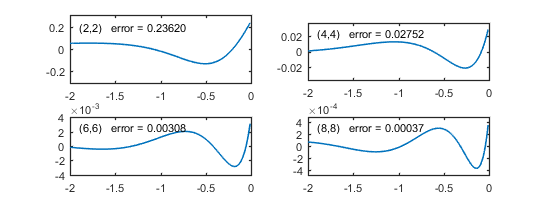
\includegraphics [width=4in]{chap25_03.png}
\begin{par}
 \vskip 1pt 
\end{par} \vspace{1em}
\begin{par}
Let us summarize these results with a theorem, which goes further to include the precise leading-order asymptotic behavior of the best approximation errors as conjectured by Magnus [1994] and proved by Aptekarev [2002].
\end{par} \vspace{1em}
\begin{par}

{\bf Theorem 25.2.  Approximation of \boldmath$e^x$ on $(-\infty,0\kern .5pt ]$.}
{\em The errors in best type $(0,n)$ and $(n,n)$ rational
approximation of $\exp(x)$ on $(-\infty,0\kern .5pt ]$ satisfy
as $n\to\infty$
$$ \lim_{n\to\infty} E_{0n}^{1/n} = {1\over 3} \eqno (25.17) $$
and
$$ E_{nn} \sim 2 \kern .4pt H^{n+1/2},
\quad H = 1/9.2890254919208\dots \eqno (25.18) $$}
\vskip -1em

\end{par} \vspace{1em}
\begin{par}

{\em Proof.}  Equation (25.17) is due to Sch\"onhage [1973] and (25.18)
to Aptekarev [2002], extending the earlier result on $n$th root
asymptotics and the constant $H$ by Gonchar and Rakhmanov [1989].
$~\hbox{\vrule width 2.5pt depth 2.5 pt height 3.5 pt}$

\end{par} \vspace{1em}
\begin{par}
We finish this chapter by showing that the numerical computation of these best approximants is surprisingly easy. The crucial matter is to note that the change of variables $$ x = a{s-1\over s+1} , \qquad  s = {a+x\over a-x} \eqno (25.19) $$ where $a$ is a positive parameter, maps the negative real axis $(-\infty,0\kern .5pt ]$ in $x$ to the interval $(-1,1]$ in $s$. Since the mapping is a rational function of type $(1,1)$, it transplants a rational function of type $(n,n)$ in $s$ or $x$ to a rational function of type $(n,n)$ in the other variable. In particular, for the approximation of $f(x) = e^x$ on $(-\infty,0\kern .5pt ]$, let us define $$ F(s) = e^{a(s-1)/(s+1)}, \quad s\in (-1,1]. \eqno (25.20) $$ A good choice of the parameter is $a=9$, which has a big effect for numerical computation in improving the conditioning of the approximation problem.  We now find we have a function that can be approximated to machine precision by a Chebyshev interpolating polynomial $p(s)$ of degree less than 50:
\end{par} \vspace{1em}
\begin{par}
 \vskip -2em 
\end{par} \vspace{1em}
\begin{verbatim}
s = chebfun('s',[-1,1]);
F = exp(9*(s-1)./(s+1));
length(F)
\end{verbatim}

        \color{lightgray} \begin{verbatim}ans =
    47
\end{verbatim} \color{black}
    \begin{par}
The Chebyshev series of $F$ decreases at a good exponential rate:
\end{par} \vspace{1em}
\begin{par}
 \vskip -2em 
\end{par} \vspace{1em}
\begin{verbatim}
clf, chebpolyplot(F), grid on
title(['Convergence of Chebyshev polynomial ' ...
       'interpolants to transplanted e^x'],FS,9)
\end{verbatim}

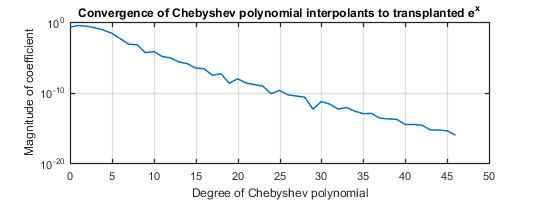
\includegraphics [width=4in]{chap25_04.png}
\begin{par}
 \vskip 1pt 
\end{par} \vspace{1em}
\begin{par}
This gives us yet another way to compute rational approximations to $e^x$ on $(-\infty,0\kern .5pt ]$: truncate this Chebyshev series in $s$, then transplant by (25.19) to get rational functions in $x$.
\end{par} \vspace{1em}
\begin{par}
Alternatively, we can get true best approximations from (25.19) by applying the Chebfun \texttt{remez} command. Here for example is the error for the best approximation of type $(8,8)$ plotted in the $s$ variable, showing 18 points of equioscillation.
\end{par} \vspace{1em}
\begin{par}
 \vskip -2em 
\end{par} \vspace{1em}
\begin{verbatim}
[P,Q,RH,err] = remez(F,8,8); R = P./Q;
hold off, plot(F-R), hold on
plot([-1 1],err*[1 1],'--k'), plot([-1 1],-err*[1 1],'--k')
xlabel('s',FS,9), ylabel error, ylim(2e-8*[-1,1])
title(['Error in type (8,8) approximation'...
       ' of transplanted e^x'],FS,9)
\end{verbatim}

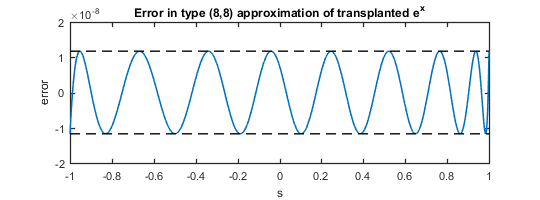
\includegraphics [width=4in]{chap25_05.png}
\begin{par}
 \vskip 1pt 
\end{par} \vspace{1em}
\begin{par}
If we plot the same curve in the $x$ variable, it's hard to see much because of the varying scale:
\end{par} \vspace{1em}
\begin{par}
 \vskip -2em 
\end{par} \vspace{1em}
\begin{verbatim}
s1 = -.999; s2 = .999; s = chebfun('s',[s1 s2]); x = 9*(s-1)./(s+1);
hold off, plot(x,F{s1,s2}-R{s1,s2}), hold on
xx = [-1e4 -1e-2];
plot(xx,err*[1,1],'--k'), plot(xx,-err*[1,1],'--k'), xlim(xx)
xlabel('x',FS,9), ylabel error, ylim(2e-8*[-1,1])
title('Error in type (8,8) approximation of e^x',FS,9)
\end{verbatim}

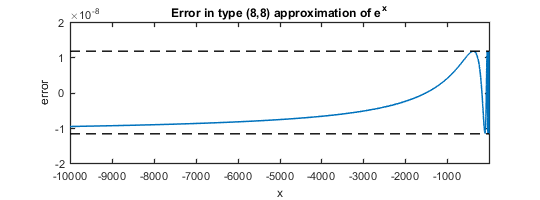
\includegraphics [width=4in]{chap25_06.png}
\begin{par}
 \vskip 1pt 
\end{par} \vspace{1em}
\begin{par}
Putting the $x$ axis on a log scale, however, makes the plot informative again:
\end{par} \vspace{1em}
\begin{par}
 \vskip -2em 
\end{par} \vspace{1em}
\begin{verbatim}
hold off, semilogx(x,F{s1,s2}-R{s1,s2}), hold on
semilogx(xx,err*[1,1],'--k'), plot(xx,-err*[1,1],'--k'), xlim(xx)
xlabel('x',FS,9), ylabel error, ylim(2e-8*[-1,1])
title('Error in type (8,8) approximation of e^x',FS,9)
\end{verbatim}

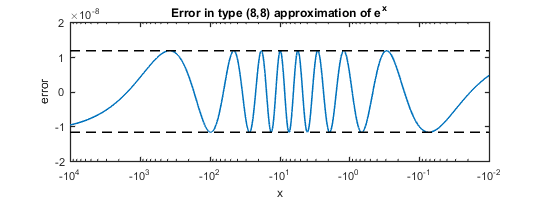
\includegraphics [width=4in]{chap25_07.png}
\begin{par}
 \vskip 1pt 
\end{par} \vspace{1em}
\begin{par}
Here is the analogous plot for type $(12,12)$ approximation:
\end{par} \vspace{1em}
\begin{par}
 \vskip -2em 
\end{par} \vspace{1em}
\begin{verbatim}
[P,Q,RH,err] = remez(F,12,12); R = P./Q;
hold off, semilogx(x,F{s1,s2}-R{s1,s2}), hold on
plot(xx,err*[1,1],'--k'), plot(xx,-err*[1,1],'--k'), xlim(xx)
xlabel('x',FS,9), ylabel error, ylim(3e-12*[-1,1])
title('Error in type (12,12) approximation of e^x',FS,9)
\end{verbatim}

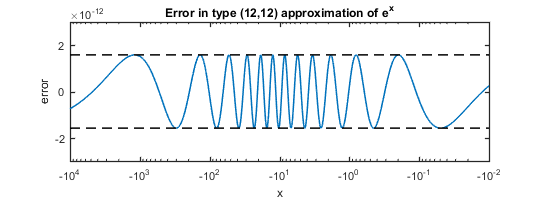
\includegraphics [width=4in]{chap25_08.png}
\begin{par}

These plots are modeled after [Trefethen, Weideman \& Schmelzer 2006],
where it is shown that Carath\'eodory--Fej\'er approximation is equally
effective and even faster than the Remes algorithm at computing these
approximations.

\end{par} \vspace{1em}
\begin{par}

\begin{displaymath}
\framebox[4.7in][c]{\parbox{4.5in}{\vspace{2pt}\sl
{\sc Summary of Chapter 25.}
Two problems involving rational functions have attracted special
attention, highlighting the power of rational approximations near
singularities and on unbounded domains. For approximating $|x|$ on
$[-1,1]$, best rational functions converge root-exponentially whereas
polynomials converge linearly.  For approximating $e^x$ on
$(-\infty,0\kern .5pt ]$, best rational functions converge geometrically
whereas polynomials do not converge at all.  Both rates of approximation
can be achieved by constructing partial fractions from trapezoid rule
approximations to certain integrals.\vspace{2pt}}}
\end{displaymath}

\end{par} \vspace{1em}
\begin{par}
\small
\parskip=2pt
{\bf Exercise 25.1.  Newton iteration for \boldmath $|x|$.}
(This problem has roots in [Roberts 1980].)
(a) Let $x$ be a number, and suppose we want to solve the
equation $r^2 = x^2$ for the unknown $r$ using Newton iteration.
Show that the iteration formula is $r^{{(k+1)}} = ((r^{(k)})^2+x^2)/2r^{(k)}$.
(b) If the initial guess is $r^{(0)} = 1$, then for $k\ge 1$, what is
the smallest $n$ for which the rational function $r^{(k)}(x)$ is of
type $(n,n)$?
(c) Use Chebfun to compute and plot the approximations
$r^{(0)}(x),...,r^{(5)}(x)$ on the interval $[-1,1]$.  What is
the sup-norm error $\||x|-r^{(k)}(x)\|$, and where is it attained?
(d) What rate of convergence does this correspond to for
$\||x|-r^{(k)}(x)\|$ as a function of $n$?  How does this compare
with the optimal rate given by Theorem 25.1?
(e) Make a semilog plot of $|\, |x|-r^{(5)}(x)| $ as a function of
$x\in [-1,1]$ and comment further on the nature of these rational
approximations.
\par
{\bf Exercise 25.2.  An elementary approximant for \boldmath$e^x$ on $(-\infty,0\kern .5pt ]$.}
A degree $n$ polynomial $p(s)$ on $[-1,1]$ can be
transplanted to a type $(n,n)$ rational function $r(x)$ on $(-\infty,0\kern .5pt ]$
by the map (25.19).  Combine this observation with Theorem 8.2
to show that type $(n,n)$ approximants to $e^x$ on $(-\infty,0\kern .5pt ]$ exist
with accuracy $O(\exp(-Cn^{-2/3}))$ for some $C>0$ as $n\to\infty$.
\par
{\bf Exercise 25.3.  Computing Halphen's constant.}
Write a short Chebfun program that computes Halphen's constant to
10 or more digits based on the condition (25.12).
\par
{\bf Exercise 25.4.  Best approximation errors for \boldmath $e^x$.}
(a) Using {\tt remez} and the change of variables (25.20), compute best approximation
errors in type $(n,n)$ approximation of $e^x$ on $(-\infty,0\kern .5pt ]$ for
$n = 0,1,\dots,13$.  Plot the results on a log scale and compare them with
estimates from the asymptotic formula (25.18).  Also on a log scale, plot
the difference between the estimates and the true errors, and comment on the
results.
(b) Repeat the computation with CF instead of {\tt remez}.  This time, plot
the different between the CF and true errors on a log scale, and comment on
the results.
\par
{\bf Exercise 25.5.  Behavior of approximants of \boldmath $|x|$ in the complex plane.}
It is shown in [Blatt, Iserles \& Saff 1988] that the type $(n,n)$ best approximants
to $|x|$ on $[-1,1]$ have all their zeros and poles on the imaginary axis
and converge to $x$ for $\hbox{Re}(x)> 0$ and to
$-x$ for $\hbox{Re}(x)< 0$ as $n\to\infty$.
Verify this result numerically by plotting $|x-r_{nn}^*(x)|$ against $\hbox{Re}(x)$
for $x\in [-1+0.5i,1+0.5i]$ for $n = 1,2,3,4$.
\par
{\bf Exercise 25.6.  Behavior of approximants of \boldmath $e^x$ in the complex plane.} It is stated in
[Stahl \& Schmelzer 2009] that the poles of best type $(n,n)$
approximations to $e^x$ on $(-\infty,0\kern .5pt ]$ move off to $\infty$ as
$n\to\infty$, and the convergence at $n$th-root rate governed by $h
\approx 1/9.28903$ applies on any compact set in the complex plane. With
this result in mind, produce contour plots in the complex $z$-plane for
the errors $|e^z - r_{nn}(z)|$ for the approximations (25.14)--(25.15)
with $n = 2, 4, 6, 8, 10$.  Does it appear likely that
these approximations too converge on all compact sets in the plane?

\end{par} \vspace{1em}



\end{document}
    
